%Notes by Harsh Mistry 
%Econ 301
%Based on Template From  https://www.cs.cmu.edu/~ggordon/10725-F12/template.tex

\documentclass[twoside]{article}
\setlength{\oddsidemargin}{0.25 in}
\setlength{\evensidemargin}{-0.25 in}
\setlength{\topmargin}{-0.6 in}
\setlength{\textwidth}{6.5 in}
\setlength{\textheight}{8.5 in}
\setlength{\headsep}{0.75 in}
\setlength{\parindent}{0 in}
\setlength{\parskip}{0.1 in}
\usepackage{amsmath,amsfonts,graphicx, color}
\newcounter{lecnum}
\renewcommand{\thepage}{\thelecnum-\arabic{page}}
\renewcommand{\thesection}{\thelecnum.\arabic{section}}
\renewcommand{\theequation}{\thelecnum.\arabic{equation}}
\renewcommand{\thefigure}{\thelecnum.\arabic{figure}}
\renewcommand{\thetable}{\thelecnum.\arabic{table}}
\newcommand{\lecture}[4]{
   \pagestyle{myheadings}
   \thispagestyle{plain}
   \newpage
   \setcounter{lecnum}{#1}
   \setcounter{page}{1}
   
   
%Info Box 
   \begin{center}
   \framebox{
      \vbox{\vspace{2mm}
    \hbox to 6.28in { {\bf Econ 301 - Microeconomic Theory 2
	\hfill Winter 2018} }
       \vspace{4mm}
       \hbox to 6.28in { {\Large \hfill Lecture #1: #2  \hfill} }
       \vspace{2mm}
       \hbox to 6.28in { {\it Lecturer: #3 \hfill Notes By: #4} }
      \vspace{2mm}}
   }
   \end{center}
   
   \markboth{Lecture #1: #2}{Lecture #1: #2}



 
}

\renewcommand{\cite}[1]{[#1]}
\def\beginrefs{\begin{list}%
        {[\arabic{equation}]}{\usecounter{equation}
         \setlength{\leftmargin}{2.0truecm}\setlength{\labelsep}{0.4truecm}%
         \setlength{\labelwidth}{1.6truecm}}}
\def\endrefs{\end{list}}
\def\bibentry#1{\item[\hbox{[#1]}]}

\newcommand{\fig}[3]{
			\vspace{#2}
			\begin{center}
			Figure \thelecnum.#1:~#3
			\end{center}
	}
	
	\graphicspath{ {images/} }

\newtheorem{theorem}{Theorem}[lecnum]
\newtheorem{lemma}[theorem]{Lemma}
\newtheorem{ex}[theorem]{Example}
\newtheorem{proposition}[theorem]{Proposition}
\newtheorem{claim}[theorem]{Claim}
\newtheorem{corollary}[theorem]{Corollary}
\newtheorem{definition}[theorem]{Definition}
\newenvironment{proof}{{\bf Proof:}}{\hfill\rule{2mm}{2mm}}
\newcommand\E{\mathbb{E}}


%Start of Document 
\begin{document}

\lecture{14}{February 28, 2018}{Jean Guillaume Forand}{Harsh Mistry}

\section{Welfare Continued}
\begin{ex} Say \(\omega^A = (3,1)\), \(\omega^B = (1, 2)\), \(u^A(x_1^A, x_2^A) = \min \{ x_1^A, x_2^A \} \), and \(u^B(x_1^B, x_2^B) = x_1^B + x_2^B\)\\
\begin{center}
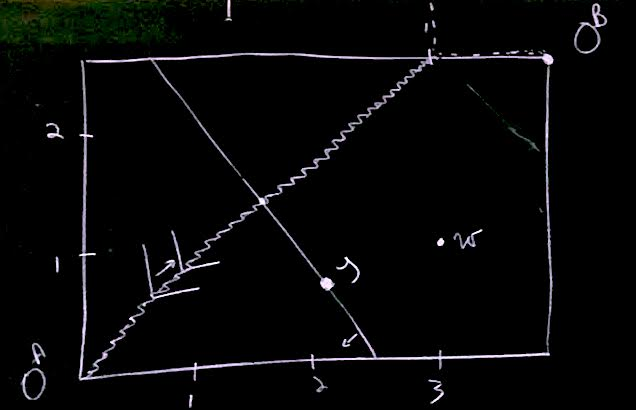
\includegraphics[scale=0.4]{25}
\end{center}
\begin{itemize}
\item Fix any allocations \(y^A\) and \(y^B\)
\item If \(y_1^A > y_2^A\), allocations \(y^A\) and \(y^B\) are pareto-dominated by allocations \(x^A =\left( \frac{y_1^A + y_2^A}{2}, \frac{y_1^A + y_2^A}{2}\right)\) and \(x^B =\left( 4-x_1^A, 3-x^A_2 \right)\)
\item Pareto set is the allocations \(x^A\) and \(x^B\) such that \(x_1^A = x_2^A\)
\end{itemize}
\end{ex}

\subsection{First Welfare Theorem}
\textcolor{red}{In-Class Numbering : 3.1} 
\begin{itemize}
\item \textbf{Question}: what is the relationship between Pareto-efficient allocations and competitive equilibrium allocations?
\end{itemize}
\begin{theorem}
FWT : Suppose that consumers' preferences are monotone and that price \(p^*\) and allocations \(x^{A*}\) and \(x^{B*}\) form a competitive equilibrium. Then \(x^{A*}\) and \(x^{B*}\) are Pareto-efficient. 
\begin{itemize}
\item Competitive Equilibria must exhaust gains from trade 
\end{itemize}
\end{theorem}

\begin{proof} By Contradiction. Suppose \(p^*\), \(x^{A*}\) and \(x^{B*}\) are a competitive equilibrium where \(x^{A*}\) and \(x^{B*}\) are not Pareto-efficient. Then there exists feasible allocations \(y^A\) and \(y^B\) such that \(u^J(y_1^J, y_2^J) \geq u^J(x_1^{J*}, x_2^{J*})\) for all \(J = 1, 2\), with one strict inequality . Say \(u^A(y_1^A, y_2^A) > u^A(x_1^{A*}, x_2^{A*})\)\\
\begin{center}
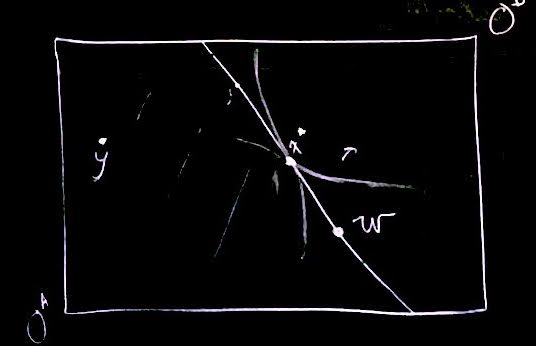
\includegraphics[scale=0.4]{26}
\end{center}
\begin{itemize}
\item Since \(y^A \succ x^{A*}\), then we must have \(p_1^* y_1^A + p_2^* y_2^A > p_1^* x_1^{A*} + p_2^* x_2^{A*}\)
\item We have \(y^A \succeq x^{B*}\)
\begin{itemize}
\item If \(y^B \succ x^{*B}\), then \(p_1 y_1^B + p_2^* y_2^B > p_1^* x_1^{B*} + x_2^{B*}\)
\item If \(y^B \sim x^{B*}\), then we must have \(p_1* x_1^{B*} + p_2^* x_2^{B*}\) [\(<\) contradicts optimality of monotonicity]
\item Then, \[\begin{aligned}p_1^* y_1^A + p_2^* y_2^A + p_1^* y_1^B  + p_2^* y_2^B & > p_1^* x_1^{A*} + p_2^* x_2^{A*} + p_1^* x_1^{B*} + p_2^* x_2^{B*} \\ & =  p_1^* \omega^A_1 + p_2^* \omega_2^A + p_1^*  \omega_2^B + p_2^* \omega_2^B \end{aligned}\]
\item So we have, \[p_1^* [y_1^A + y_1^B - \omega_1^A - \omega^B_2] + p_2^* [y^A_2 + y_2^B - \omega_2^A - \omega_2^B] > 0\]
\textbf{\textcolor{red}{Contradiction}}, feasibility of \(y^A, y^B\) is violated. Basically, this statement implies we have more of a good than what actually exists. \\

\textbf{Note : } Proof is included to supplement the First Welfare Theorem to make understanding it easier. The proof itself, despite the awesomeness of mathematical proofs,  is not a testable topic. It can essentially be ignored.
\end{itemize}
\end{itemize}
\end{proof}

\begin{itemize}
\item First Welfare Theorem says that competitive equilibrium allocations reproduce the outcomes of \underline{some} bargaining protocol
\item In bargaining, computing outcomes (P-E Allocations) requires a lot of information about consumers preferences and aggregate endowments.
\item Markets only require consumers to know their own preferences and endowments. 
\item Prices aggregate economy-wide information. 
\end{itemize}


\end{document}





